% BENCHMARKS    --------------------------------------------
\section{Benchmarks}
    Considering the several aspects of software performance, here are highlighted some micro-benchmarks which can impact on the performance of the software and could change the performance of software throughout the releases.
    
    \textit{inline}\\
    The inline functions are a C++ enhancement feature to increase the execution time of a program. Functions can be compiled as inline automatically, or can be declared by the programmer as inline functions. The compiler replaces the definition of inline functions at compile time instead of referring function definition at runtime.
    
    However, those functions do not always improve the performance and can deteriorate the performance \cite{inline_site}. To evaluate this claim, we tested this feature with several possibilities: strings, integers, structs, vectors, and classes. Using the inline made the performance better for all of them, except for std::string operations. 
    
    The reason for this difference possibly is related with the dynamic allocation time of strings in C++ as explored by \cite{optc++}. We did several tests with different data structures and objects, and strings seems the more effected by this effect.
    
    After investigation, we came to the conclusion that the root cause of this performance degradation is the influence of cache misses in the operations with string inside inline functions.
    
    Comparing the performance of inline functions and regular functions, the results of the benchmarks are shown in the Figures \ref{fig:notinline} and \ref{fig:inline}. For thousand runs, the average, the mean and the median were high in comparison to use the not inline implementation.
    
    \textit{template functions} \\
     Template functions can decrease the performance of a software.
     According to Jacob B. Matthews, from the university of Chicago, \cite{chicago}, the use of templates decrease efficiency of the C++ compiler's.
     
     
    \textit{virtual functions} \\
     The use of virtual functions has a cost for the dispatching. The work of \cite{dispatch} shows the overhead related with dispatching on C++ codes.
     
    \begin{figure}[h]
      \centering
        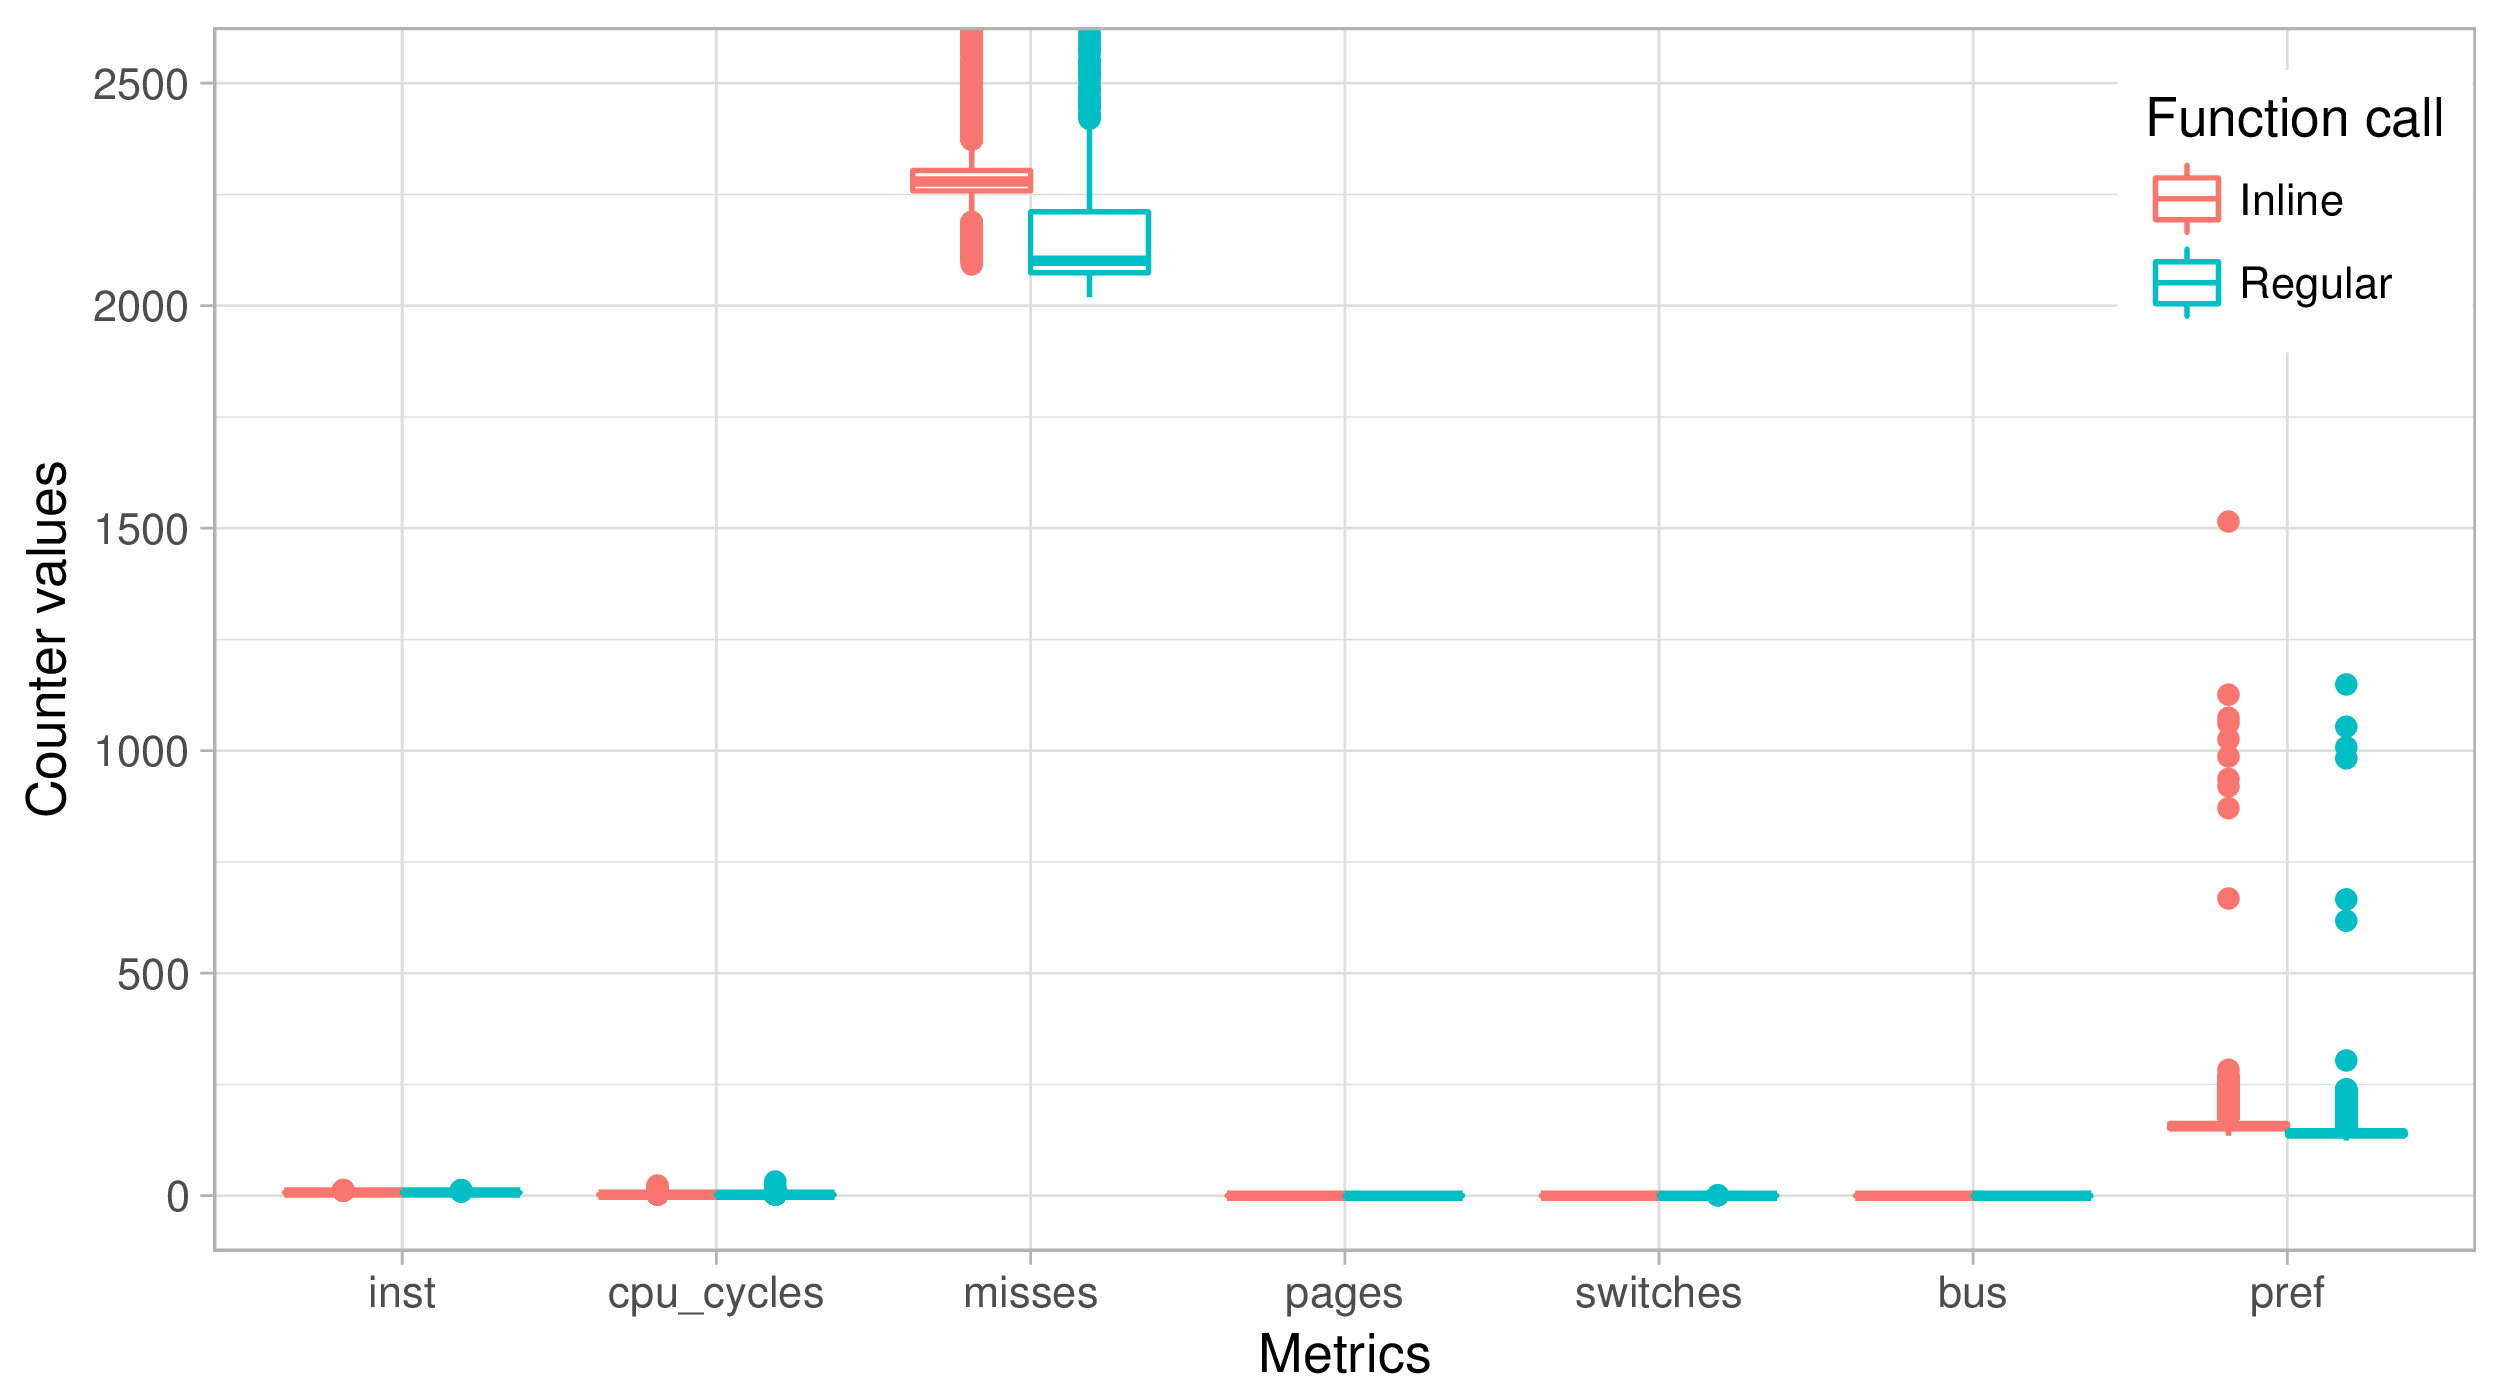
\includegraphics[width=0.47\textwidth]{figures/boxplots-inline-vs-regular.png}
        \caption{Counter Metrics for Inline and Regular function calls}
        \label{fig:notinline}
    \end{figure}
    
    \begin{figure}[h]
      \centering
        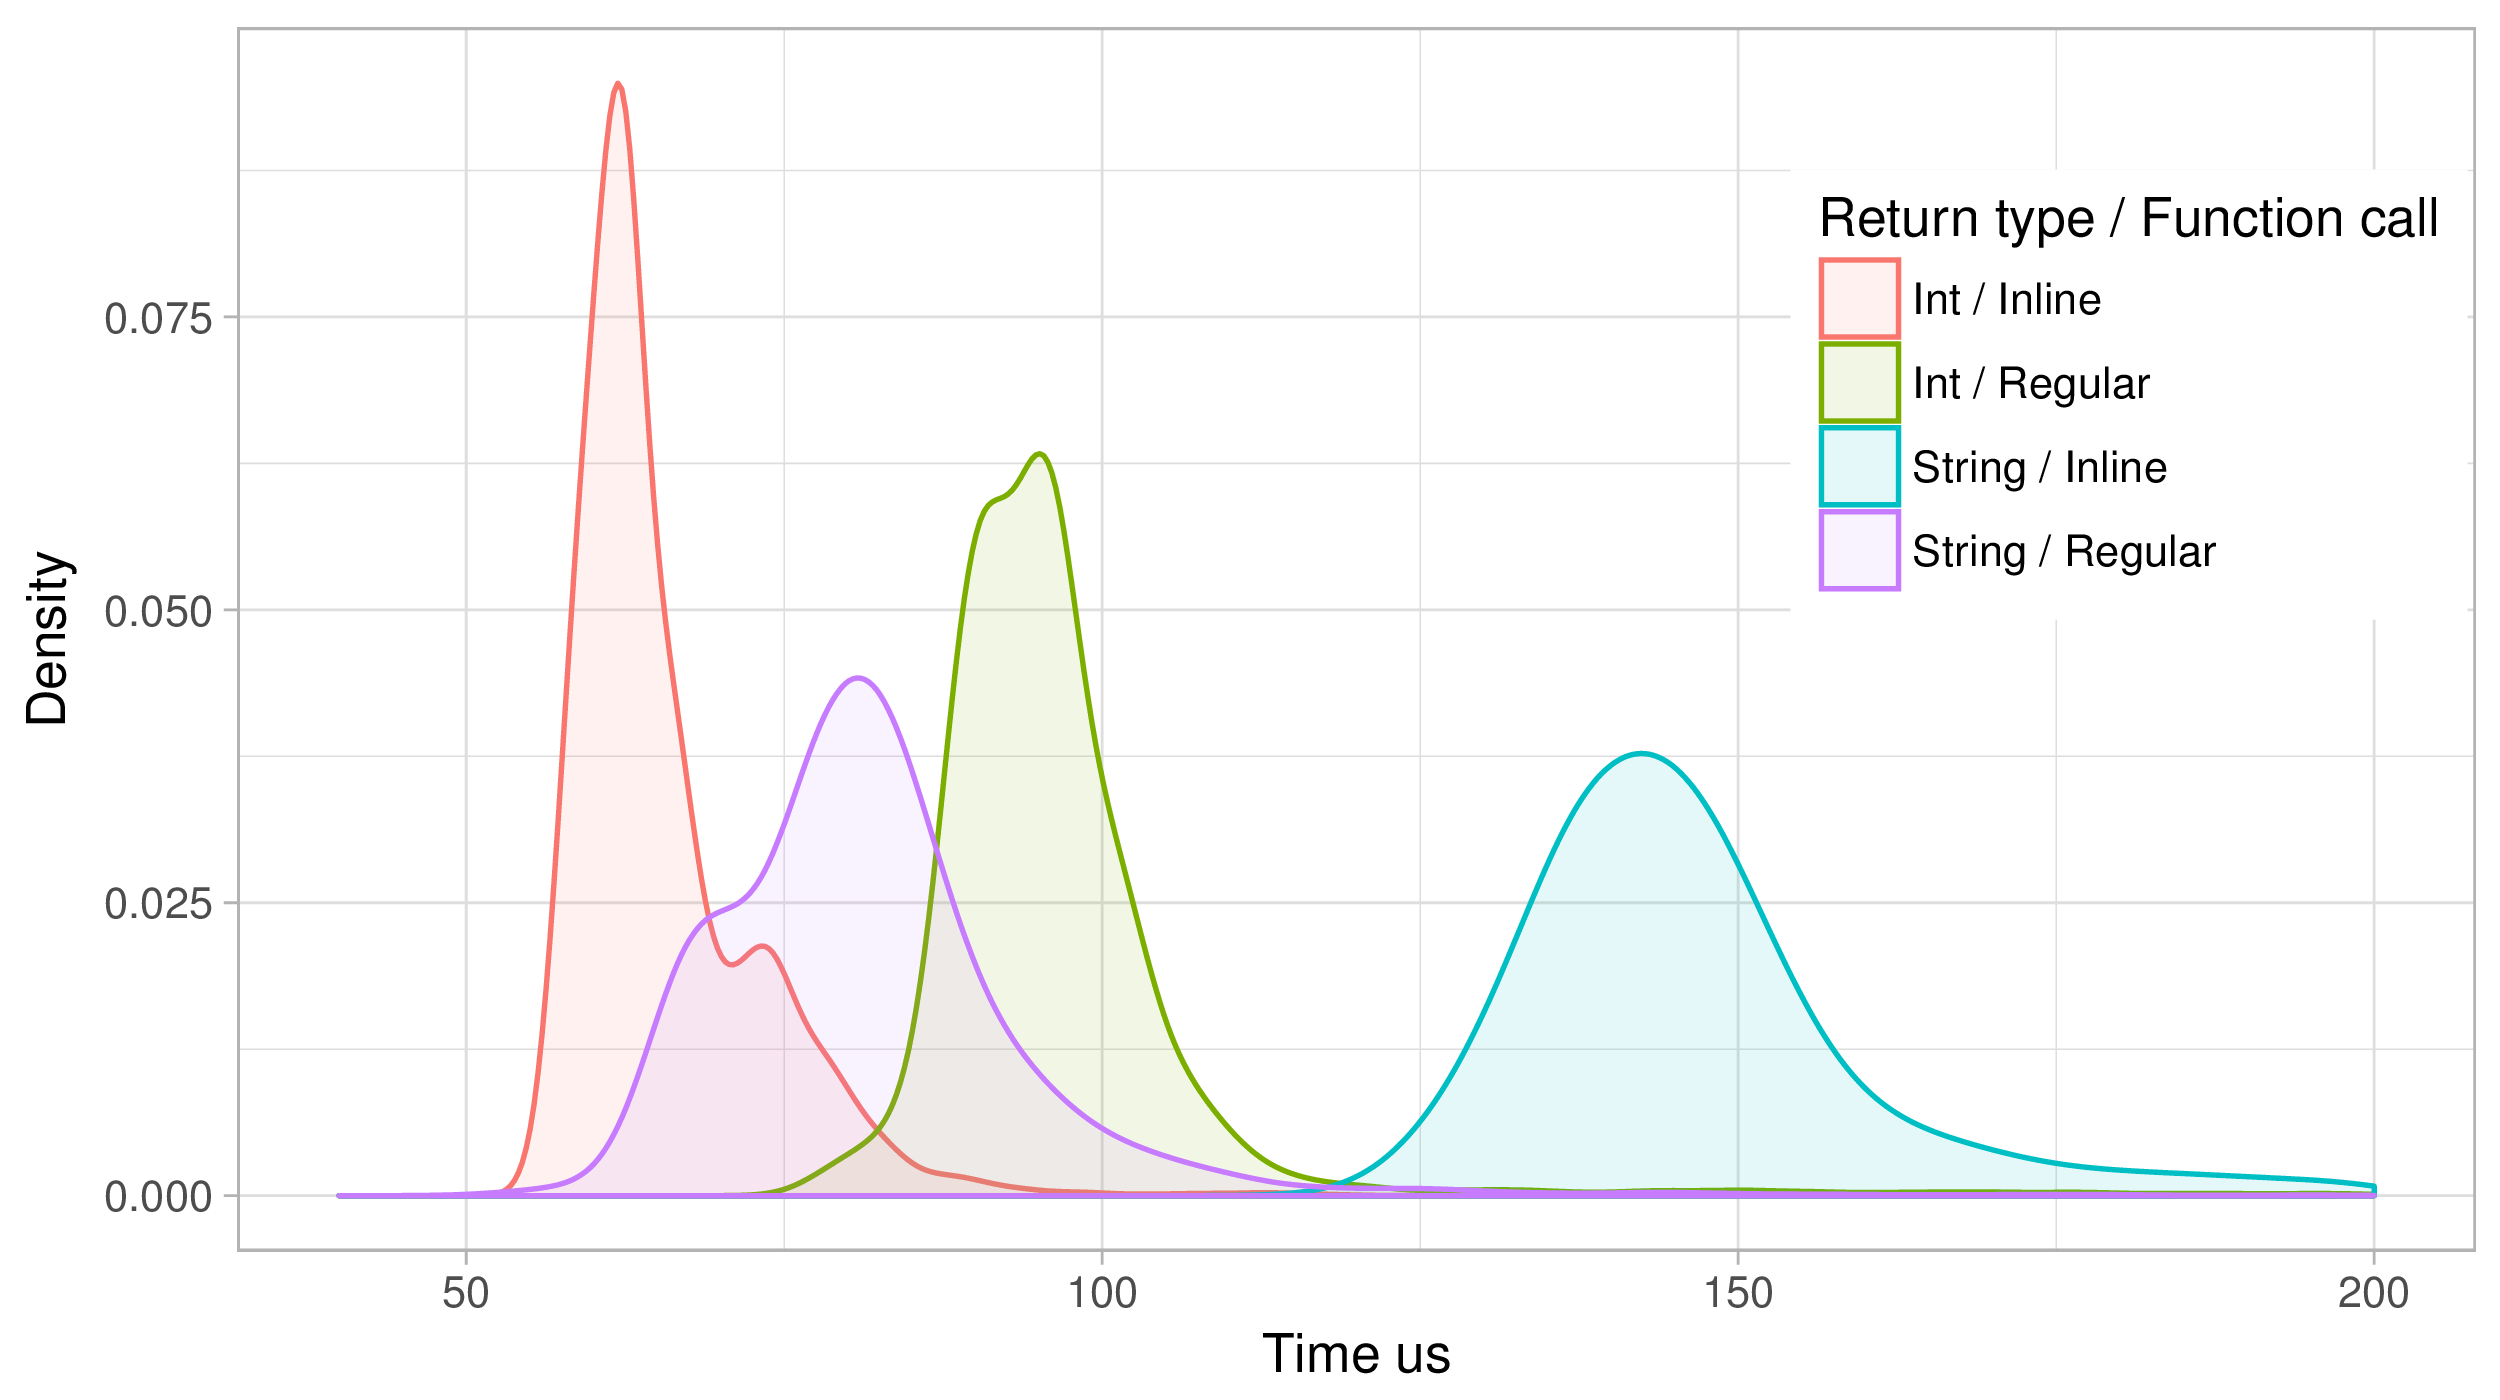
\includegraphics[width=0.47\textwidth]{figures/density-inline-vs-regular.png}
        \caption{Distribution of Inline vs Regular functions using String and Integer as return types}
        \label{fig:inline}
    \end{figure}
    
    
    \section{Illustrative Example}
    
\textbf{Open Close}
    To illustrate the approach used, we developed a small code which does several times the process of opening a file subsequently. The code was instrumented with -finstrument functions and this gave the possibility to run the code using Lttng-UST.
    When execute this code several times, some executions have a different behaviour, which we call outliers.
    Using our approach, first we record the executing metrics of the program, then the automated cluster technique is applied, finally we compare the groups: slow executions and fast executions. We deduced that the problem was related with the wait-cpu time metric on the slow executions.
    
    The figure \ref{fig:group} demonstrates the grouping mechanism, which segregated the executions in two groups, the association rule related all the slow executions with wait-cpu group 2 and the fast executions with wait-cpu group 1. The association showed that the wait-cpu was the cause for this difference of the groups.
    
     \begin{figure}[h]
      \centering
        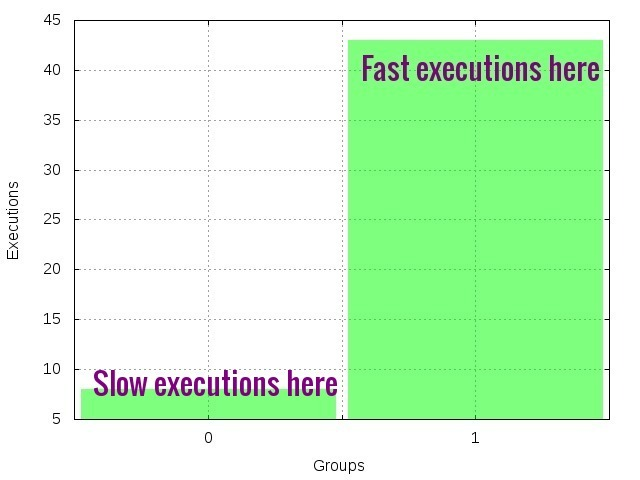
\includegraphics[width=0.50\textwidth]{figures/grouping.jpg}
        \caption{Comparing executions of Open program}
        \label{fig:group}
    \end{figure}

    
    
\textbf{Executions}
    All experiments were done in a computer with a quad-core Intel® CoreTM i7-3770 CPU running at 3.4 GHz, 16 GB of DDR3 memory and a 7200 RPM hard drive. The Linux kernel version was 3.13.0-49 while the LTTng version was 2.6.0.
% \subsection{\textbf{Scheduler Interference}}
  
% \subsubsection{Summary}
%     A process is executed with lower priority than another, which is triggered on regular intervals. The scheduler plays its role to change the process order at regular times on Linux systems.
    
% \subsubsection{Approach}
%     Our approach was to run the process several times to trigger the conflict with a task with higher priority. While running it, we recorded the tracing data. Then, we executed our clustering analysis and classified the data in several groups. Were able to find that on the fast runs the execution took: x milliseconds. However, on not normal executions - slow executions.
    
% \subsubsection{Results}
%      Were able to find that on the fast runs the execution took: x milliseconds. However, on not normal executions - slow executions. The automated comparison showed that the main difference was on the x function.

    

% \subsection{\textbf{Regression Comparison}}
    
% \subsubsection{Summary}
%     A new feature was added on the new software version and the performance regressions tests are showing a slightly performance difference with a feature, which uses inline functions.
    
% \subsubsection{Approach}
%     Our approach was to run the software several times with the function using and not using inline. The tool was applied from the tracing data. The benchmarks used showed that strings operations with inline can have a difference performance.
    
% \subsubsection{Results}
%     The functions using inline were a little worst in terms of performance to non inline versions. The classification result showed that inline were related with a larger number of cache misses indeed.

%     Figure \ref{fig:case1}, shows the grouping results relating the cache misses with the slow executions groups.
    
%     \begin{figure}[h]
%           \centering
%             \includegraphics{figures/inline.png}
%             \caption{Case study Regression - showing differences on the runs using inline functions and not inline}
%             \label{fig:case1}
%     \end{figure}